%=========================================================
\chapter{Modelo del Alcance}
\label{cap:reqUsr}

	En este capítulo se modela el alcance del sistema. Se presentan inicialmente los Actores involucrados y sus requerimientos. Después se presentan los requerimientos funcionales se presenta el modelo Físico y Lógico del sistema.


%---------------------------------------------------------
\section{Modelado de Usuarios}
%\cdtInstrucciones{
%	Identifique los actores que estarán involucrados en los procesos relacionados con el sistema para esta iteración de desarrollo. Ponga énfasis en los procesos involucrados.
%}

\subsection{Organigrama de la Empresa}



\begin{figure}[htbp]
	\begin{center}
		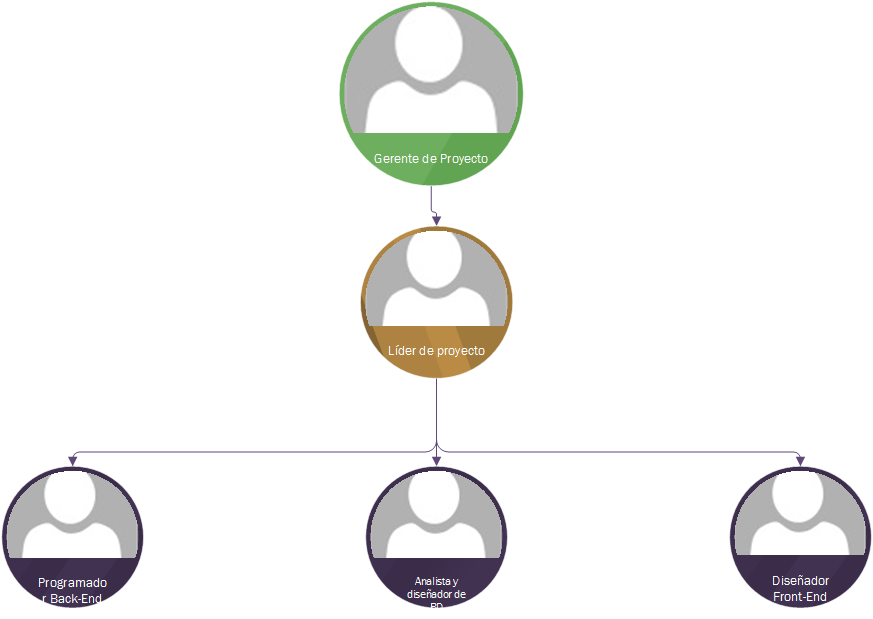
\includegraphics[width=.8\textwidth]{images/organigramaEm}
		\caption{Organigrama mal debe ser el de la empresa}
		\label{fig:organigrama}
	\end{center}
\end{figure}

%=========COPIA DESDE AQUI PARA AGREGAR A TU ACTOR=========
%---------------------------------------------------------
\begin{Usuario}{\subsection{Jefe de Inmobiliario}}{
		Es el encargado de todas las operaciones que tengan que ver con con la sucursal, como lo son áreas, actividades y propiamente las sucursales, supervisa que los datos estén actualizados del inmueble.
	}
	\item[Responsabilidades:] \cdtEmpty
	\begin{itemize}
		\item Supervisar la información de actividades, áreas y sucursales.
		\item Agrega o modifica los datos.
	\end{itemize}
	
	\item[Perfil:] \cdtEmpty
	\begin{itemize}
		\item Amplia experiencia en el ramo.
		\item Licenciatura como mínimo.
	\end{itemize}
	\item[Procesos en los que participa:] \cdtEmpty
	\begin{itemize}
		\item PC-V01 Aprobar la agregación de nuevas actividades.
		\item PC-V02 Supervisar el ingreso a la sucursal
		\item PC-V03 Elaborar informe incidencias en la sucursal.
	\end{itemize}
\end{Usuario}

%---------------------------------------------------------
%=======HASTA AQUI TERMINA PARA AGREGAR A TU ACTOR========


%---------------------------------------------------------
\section{Requerimientos de usuario}

%\cdtInstrucciones{
%	Identifique y describa los requerimientos funcionales del sistema señalando: id, nombre, descripción y prioridad.
%}

\begin{table}[htbp!]
	\begin{requerimientosU}
		\FRitem{RU1}{Registro de clientes}{El usuario requiere llevar un registro actualizado de todos los clientes para su seguimiento, atención teniendo por datos el nombre completo, domicilio, correo, curp, teléfono, número de emergencia, fecha de nacimiento y datos medicos como estatura, peso, alergias y enfermedades crónicas, si toma algún medicamento.}{1}{\PLAN}
		
		\FRitem{RU2}{Registro de áreas}{El usuario requiere llevar un registro actualizado de todas las áreas que tenga la sucursal teniendo como datos la capcidad máxima de personas, encargado del área, actividades impartidas, la(s) sucursal(es) donde se encuentra y horario(s).}{1}{\PLAN}
		
		\FRitem{RU3}{Registro de actividades}{El usuario requiere llevar un registro actualizado de todas las actividades que tenga la sucursal teniendo como datos nombre de a actividad, dia y hora en que se imparte, que instructor tiene, cuantos estan inscritos, etc.}{1}{\PLAN}
		
		\FRitem{RU4}{Registro de sucursal}{El usuario requiere llevar un registro actualizado de todas las sucursales que haya en la franquicia.}{1}{\PLAN}
		
		\FRitem{RU5}{Planeación de personal}{El usuario requiere llevar un registro de los roles que tiene cada empleado de la sucursal.}{1}{\PLAN}
		\FRitem{RU6}{Visualización de infromación}{El usuario requiere ver la información almacenada la información desplegando pantallas.}{1}{\PLAN}
		\FRitem{RU7}{Registro de pago}{El usuario requiere ver la información de los clientes que realizan su pago.}{1}{\PLAN}
		\FRitem{RU8}{Aviso de pago}{El usuario requiere informar al cliente de su próximo pago.}{1}{\PLAN}
		\FRitem{RU9}{Registro de ingreso}{El usuario requiere ver la información de quién ingresa a la sucursal.}{1}{\PLAN}
		
	\end{requerimientosU}
	\caption{Requerimientos funcionales del sistema.}
	{\footnotesize\em Para leer correctamente esta tabla vea la leyenda en la Tabla~\ref{tbl:leyendaRF} en la página~\pageref{tbl:leyendaRF}.}
	\label{tbl:reqFunc}
\end{table}



%---------------------------------------------------------
\section{Especificación de plataforma}	

\cdtInstrucciones{
	Coloque un diagrama y su descripción para aclarar el tipo de solución propuesta. \\
	
	En esta sección se debe aclarar:}
	
	\begin{description}
		\item[Tipo de sistema:] Aplicación web.
		\item[Software requerido:] --.
		\item[Hardware requerido:] Tener como mínimo windows 7 o distribución de linunx a partir de la versión --.
		\item[servicios:] --.
	\end{description}


\begin{figure}[htbp!]
	\begin{center}
		\fbox{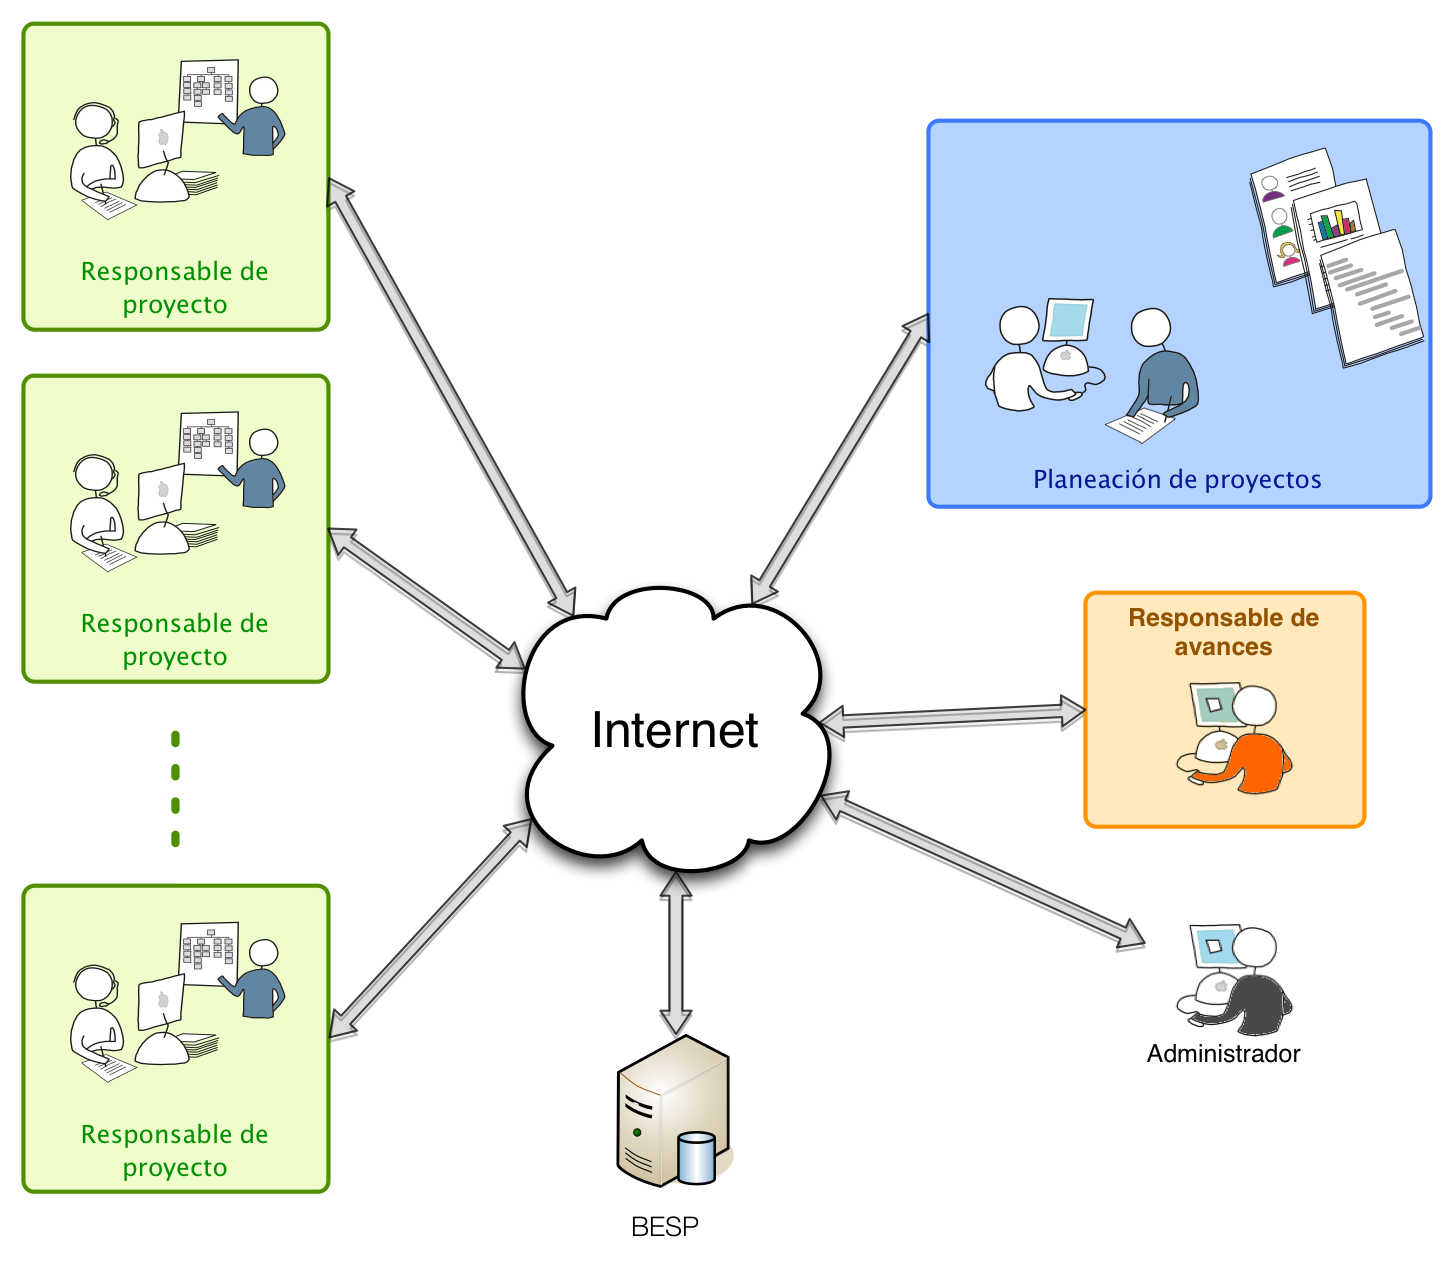
\includegraphics[width=.6\textwidth]{images/arquitectura}}
		\caption{Arquitectura del sistema.}
		\label{fig:arquitectura}
	\end{center}
\end{figure}

En la figura~\ref{fig:arquitectura} se describe la estructura del sistema, en ella se detalla ...